\documentclass[letterpaper]{article}
\usepackage[utf8]{inputenc}
\usepackage[spanish]{babel}
\usepackage{amssymb, amsmath}
\usepackage{graphicx}
\usepackage{lipsum}
\usepackage{dsfont}
\usepackage[margin=1.5cm,
vmargin={1cm,0.3cm},
includefoot]{geometry}
\usepackage{setspace}
\usepackage{subcaption}
\usepackage{tocloft}
\usepackage{upgreek}
\usepackage{amsthm}
\usepackage{graphicx}
\usepackage{paralist}
\usepackage{fancyhdr}
\usepackage{lmodern}
\usepackage{tcolorbox}
\usepackage{color}
\usepackage{tikz}
\tcbuselibrary{skins,breakable}
\pagestyle{fancy}

\renewcommand{\headrulewidth}{0.4pt}
\renewcommand{\footrulewidth}{0.4pt}

\providecommand{\abs}[1]{\left|#1\right|}
\providecommand{\norm}[1]{\left|\left|#1\right|\right|}														  
\newcommand{\tq}{ \quad \cdot  \backepsilon \cdot \quad }

\newcommand{\ld}{\lim\limits_{x \to 0^{+}}}

\newcommand{\li}{\lim\limits_{x \to 0^{-}}}

\newcommand{\la}{\lim\limits_{x \to a}}

\newcommand{\R}{\mathds{R}}
\newcommand{\Q}{\mathds{Q}}

\newcommand{\Z}{\mathds{Z}}

\newcommand{\N}{\mathds{N}}

\renewcommand{\P}{\mathcal{P}}

\newcommand{\Po}{\mathds{P}_2(\mathds{R})}

\renewcommand{\*}{\cdot}

\makeatletter
\renewcommand*\env@matrix[1][*\c@MaxMatrixCols c]{%
	\hskip -\arraycolsep
	\let\@ifnextchar\new@ifnextchar
	\array{#1}}
\makeatother

\newtheorem{theorem}{Teorema}[section]
\theoremstyle{definition}
\newtheorem{definition}{Definición}

\begin{document}
\setlength{\unitlength}{1cm}
\thispagestyle{empty}
\begin{picture}(19,3)
\put(-0.5,1.2){
\includegraphics[scale=.20]{unam1.png}}
\put(16,1){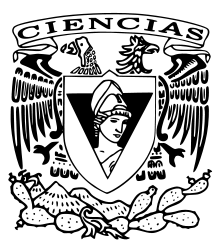
\includegraphics[scale=.29]{fciencias1.png}}
\end{picture}

\begin{center}
	\vspace{-114pt}
	\textbf{\large Álgebra Superior I}\\
	\textbf{ Semestre 2020-2}\\
	Prof. Alejandro Dorantes Aldama\\
	Ayud. Elmer Enrique Tovar Acosta \\
	Ayud. Alejandro Ríos Herrejón \\
	\textbf{Reposición examen I}
\rule{19cm}{0.2mm}
	\vspace{-0.7cm}
	\begin{center}
Kevin Ariel Merino Peña\footnote[2]{Número de cuenta: 317031326}
	\end{center}
	\vspace{-0.5cm}
\rule{19cm}{0.2mm}
\end{center}
 %%%%%%%%%%%%%%%%%%%%%%%%%%%%%%%%%%%%%%%%%%%%
 %			|	EJERCICIO 4					%
 %			|	ARIEL						%	
 %%%%%%%%%%%%%%%%%%%%%%%%%%%%%%%%%%%%%%%%%%%%
\noindent4. Sean A,B conjuntos. Demuestre que las siguientes son equivalentes:
\begin{enumerate}
	\item $ A \subset B $
	\item $ A \cap B = A $
	\item $ A \cup B = B $
	\item $ A \backslash B = \varnothing $
\end{enumerate}
$ 1) \implies 2) $ Supongamos $ A \subseteq B $, por demostrar: $ A \cap B = A $.
\\ $\subseteq]  $
\begin{align*}
	&\text{Supongamos que } & a \in A&\cap B  \\
	&\text{Por definición de intersección } & a \in A &\land a \in  B \\
	&\text{Particularmente } a &\in A \\
	& &  A \cap B &\subseteq A 
\end{align*}
$\supseteq]  $
\begin{align*}
	&\text{Supongamos } & a &\in A\\
	&\text{Por hipótesis } & A &\subseteq B \\
	&\text{Parrticularmente } & a &\in B \\
	&\text{Entonces } & a \in B & \land a \in A\\
	&\text{\textit{i.e.} } & a &\in A \cap B \\
	&\text{ } & A &\subseteq A \cap B 
\end{align*}
\begin{center}
	Como tenemos $ A \subseteq A \cap B  $ y $ A \supseteq A \cap B  $
	$$ \therefore \qquad A = A \cap B  $$
\end{center}

 %%%%%%%%%%%%%%%%%%%%%%%%%%%%%%%%%%%%%%%%%%%%
 %			|	EJERCICIO 8					%
 %			|	ARIEL						%	
 %%%%%%%%%%%%%%%%%%%%%%%%%%%%%%%%%%%%%%%%%%%%
\noindent8. Sean $ A = \{ 1,2,3 \} $ y $ B =\{ 1,2,3,4 \} $. Encuentre todas las parejas ordenadas de $ A \times B $.\\

 %%%%%%%%%%%%%%%%%%%%%%%%%%%%%%%%%%%%%%%%%%%%
 %			|	EJERCICIO 9					%
 %			|	ARIEL						%	
 %%%%%%%%%%%%%%%%%%%%%%%%%%%%%%%%%%%%%%%%%%%%
\noindent9. Sean $ A = \{ 1,2, \dots, n \} $ y $ B = \{ 1,2, \dots, m \} $. Demuestre que el producto $ A \times B $ tiene $ nm $ elementos. Sugerencia: ¿Cuántas parejas tienen como primera coordenada 1?, ¿y 2?\\



 %%%%%%%%%%%%%%%%%%%%%%%%%%%%%%%%%%%%%%%%%%%%
 %			|	EJERCICIO 16				%
 %			|	ARIEL						%	
 %%%%%%%%%%%%%%%%%%%%%%%%%%%%%%%%%%%%%%%%%%%%
\noindent16. Encuentre la imagen de las siguientes funciones:
\begin{itemize}
	\item $ f : \N \to \N $ dada por $ f(n) = n + 1 $.
	\item $ f : \N \to \N $ dada por $ f(n) = n^2 + 1 $.
	\item $ f : \Z \to \N $ dada por $ f(n) = n^2 + 1 $.
\end{itemize}


 %%%%%%%%%%%%%%%%%%%%%%%%%%%%%%%%%%%%%%%%%%%%
 %			|	EJERCICIO 17				%
 %			|	ARIEL						%	
 %%%%%%%%%%%%%%%%%%%%%%%%%%%%%%%%%%%%%%%%%%%%
\noindent17. Sean $ f, g: \R \to \R $ dadas por $ f(x) = x + 1 $ y $ g(x) = x^2 $. Calcule $ f \circ g $ y $ g \circ f $.\\
\textbf{Nota:} Para los ejercicio 18, por "Encontrar funciones" se entiende dat todos los elementos que determinan una función, es decir, dominio, codomino y la regla de correspondencia.\\

 %%%%%%%%%%%%%%%%%%%%%%%%%%%%%%%%%%%%%%%%%%%%
 %			|	EJERCICIO 21				%
 %			|	ARIEL						%	
 %%%%%%%%%%%%%%%%%%%%%%%%%%%%%%%%%%%%%%%%%%%%
\noindent21. Como siempre, los símbolos $ \N $ y $ \Q $ denotarán al conjunto de número naturales y al conjunto de números racionales, respectivamente, ¿Es cierto que 
\[ R:= \left\lbrace \left(\dfrac{m}{n}, \dfrac{1}{n}\right): m, n \in \N \right\rbrace \]
es una función de $ \Q $ en $ \Q $?\\


\end{document}